% Arquivo editável que gera o pdf
% Copyright (C) 2018  Daniel Saad Nogueira Nunes (daniel.nunes@ifb.edu.br)

% This program is free software: you can redistribute it and/or modify
% it under the terms of the GNU General Public License as published by
% the Free Software Foundation, either version 3 of the License, or
% (at your option) any later version.

% This program is distributed in the hope that it will be useful,
% but WITHOUT ANY WARRANTY; without even the implied warranty of
% MERCHANTABILITY or FITNESS FOR A PARTICULAR PURPOSE.  See the
% GNU General Public License for more details.

% You should have received a copy of the GNU General Public License
% along with this program.  If not, see <http://www.gnu.org/licenses/>.


\documentclass{aula-ifb}
\usepackage{subfig}

% Insira os dados aqui
\author{Maxwell Borges Bezerra\\ 
\small{Orientador: prof. Daniel Saad}}
\title{Definição, Estudo e Implementação de um Sistema de Divulgação de Informações Integrado do IFB}
%\subtitle{Graduação em Bacharelado em Ciência da Computação}
\institute{Instituto Federal de Brasília, Câmpus Taguatinga}
\date{26 de Junho de 2018}



\begin{document}
\maketitle
\section{Introdução}
\begin{frame}{Organização}
\begin{itemize}
\item Introdução
\item Trabalhos relacionados
\item Graph API
\item SID
\item Resultados
\item Trabalhos futuros
\end{itemize}
\end{frame}

\subsection{Marketing}
\begin{frame}{Marketing}
\begin{center}
O marketing tem por objetivo, persuadir as pessoas a tomar determinadas ações que são desejadas pela divulgação.
\end{center}
\end{frame}

\begin{frame}{Marketing}
	\begin{figure}[h]
  		\centering
  		\subfloat[Revistas]{
    		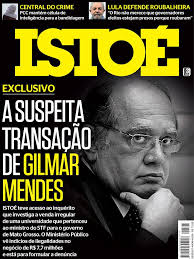
\includegraphics[height=2cm]{figuras/revista.png}
  		}
  \quad %espaco separador
  \subfloat[Jornais]{
    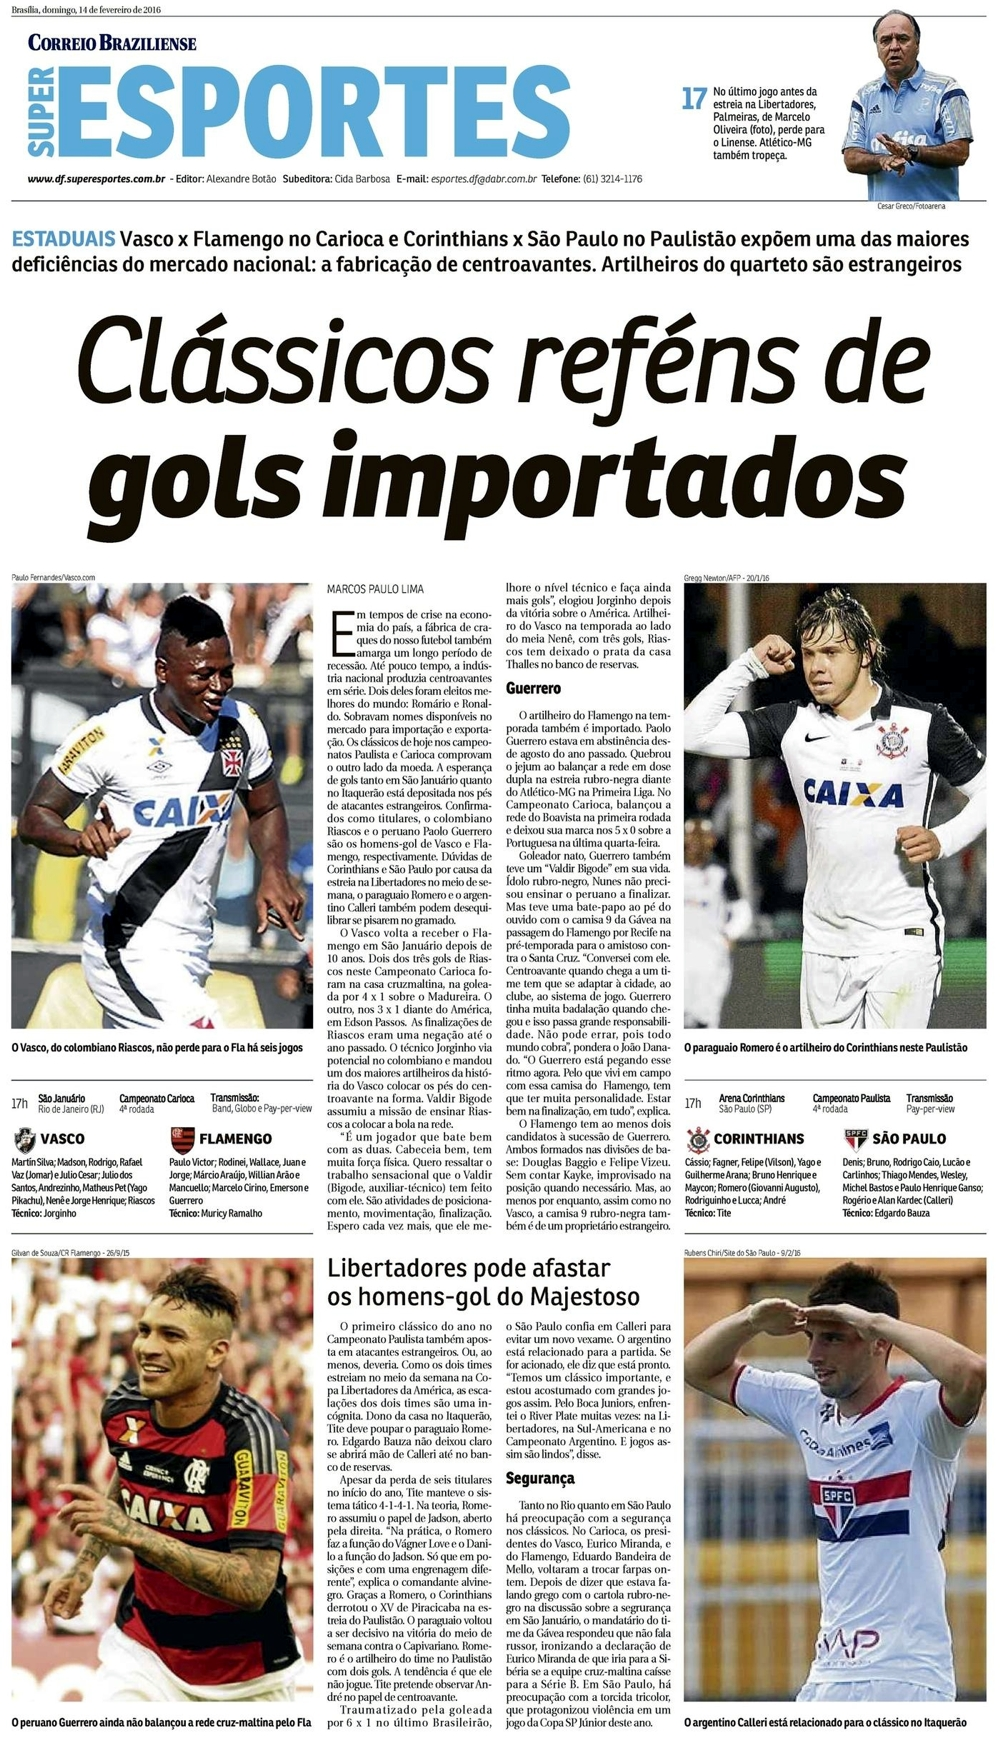
\includegraphics[height=3cm]{figuras/jornal.png}
  }
  \quad %espaco separador
  \subfloat[Outdors]{
    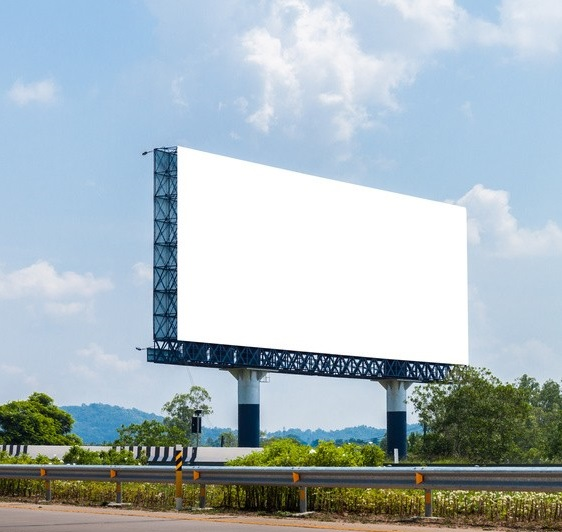
\includegraphics[height=2cm]{figuras/outdor.png}
    \label{fig3b}
  }
  \quad %espaco separador
  \subfloat[Televisões]{
    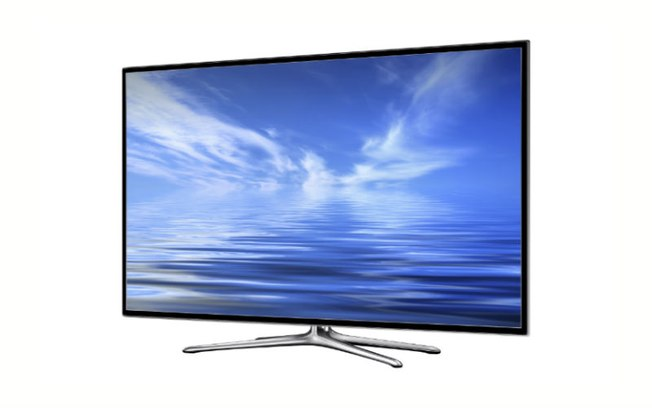
\includegraphics[height=2cm]{figuras/televisao.png}
    \label{fig3b}
  }
   \caption{Principais meios de divulgação}
	\label{fig1}
\end{figure}
\end{frame}

\subsection{Marketing Digital}
\begin{frame}{Marketing Digital}
\begin{center}
Publicidade tem tudo a ver com influenciar pessoas, tornando as publicações melhor assimilável e com a união da tecnologia, se cria um novo panorama de marketing  \cite{ryan2016}\\
\vspace{20px}
Mídias sociais são páginas de Internet onde os usuários são ao mesmo tempo produtor e consumidor, incluindo as interações com os usuários.  \cite{torres2000} 
\end{center}
\end{frame}

\begin{frame}{Marketing Digital}
\begin{figure}[h]
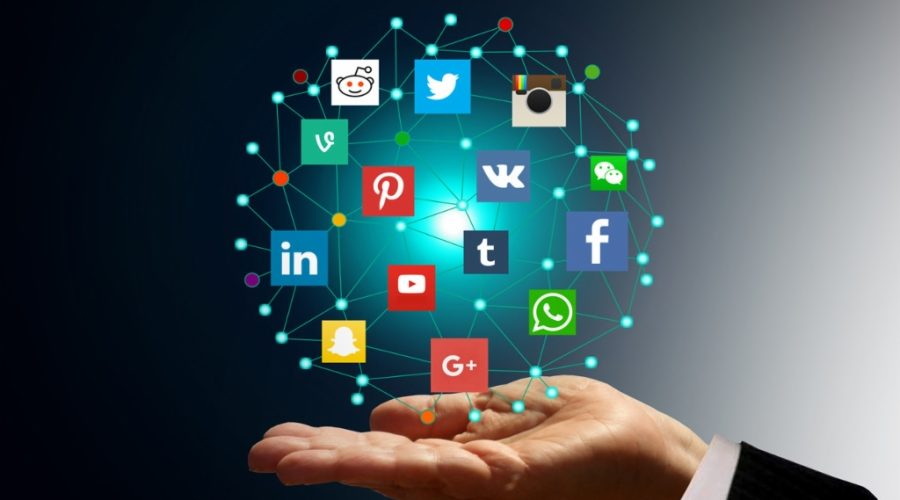
\includegraphics[width=8cm]{figuras/marketingdigital.png}
\caption{Marketing Digital \cite{figura1}}
\label{fig:siteifb}
\end{figure}
\end{frame}

\subsection{Sinalização Digital}
\begin{frame}{Sinalização Digital}
\begin{center}
Transmissão de conteúdo, via Internet, à televisões ou painéis dos mais diversos tamanhos e nos mais diversos locais. \cite{machado2010}\\

\vspace{20px}
Sinalização digital pode ser usada como alternativa aos outdoors, que poluem visualmente grandes cidades. \cite{cintra2010}

\end{center}
\end{frame}

\begin{frame}{Sinalização Digital}
\begin{figure}[h]
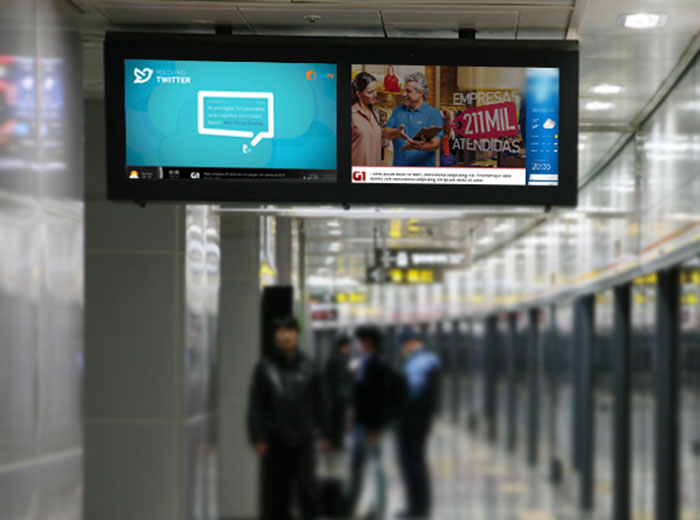
\includegraphics[width=8cm]{figuras/sinalizacaodigital.png}
\caption{Sinalização Digital \cite{figura2}}
\label{fig:siteifb}
\end{figure}
\end{frame}

\subsection{Definição do problema}
\begin{frame}{Atuais meios online}
\begin{figure}[h]
  \centering
  \subfloat[Página WEB]{
    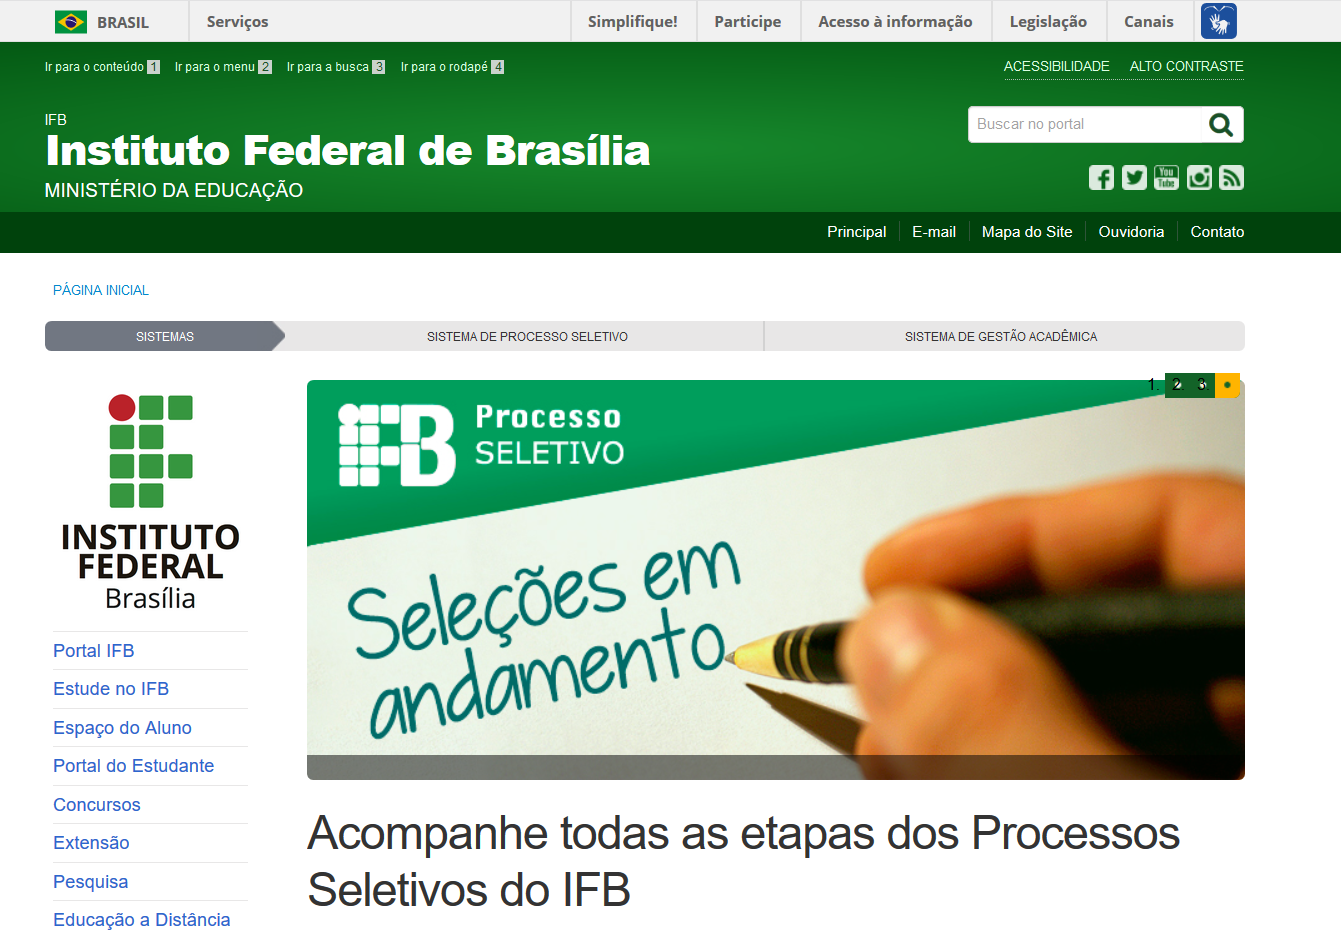
\includegraphics[height=3.5cm]{figuras/siteifb.png}
    \label{fig03a}
  }
  \quad %espaco separador
  \subfloat[Página Facebook]{
    
\includegraphics[height=3.5cm]{figuras/facebookifb.png}
    \label{fig3b}
  }
  \caption{Meios de divulgação online no IFB}
\label{fig1}
\end{figure}
\end{frame}

\begin{frame}{Atuais meios fisicamente no IFB}
\begin{figure}[h]
  \centering
  \subfloat[Panfletos]{
    
\includegraphics[height=3cm]{figuras/panfletos.png}
    \label{fig03a}
  }
  \quad %espaco separador
  \subfloat[Painéis]{
    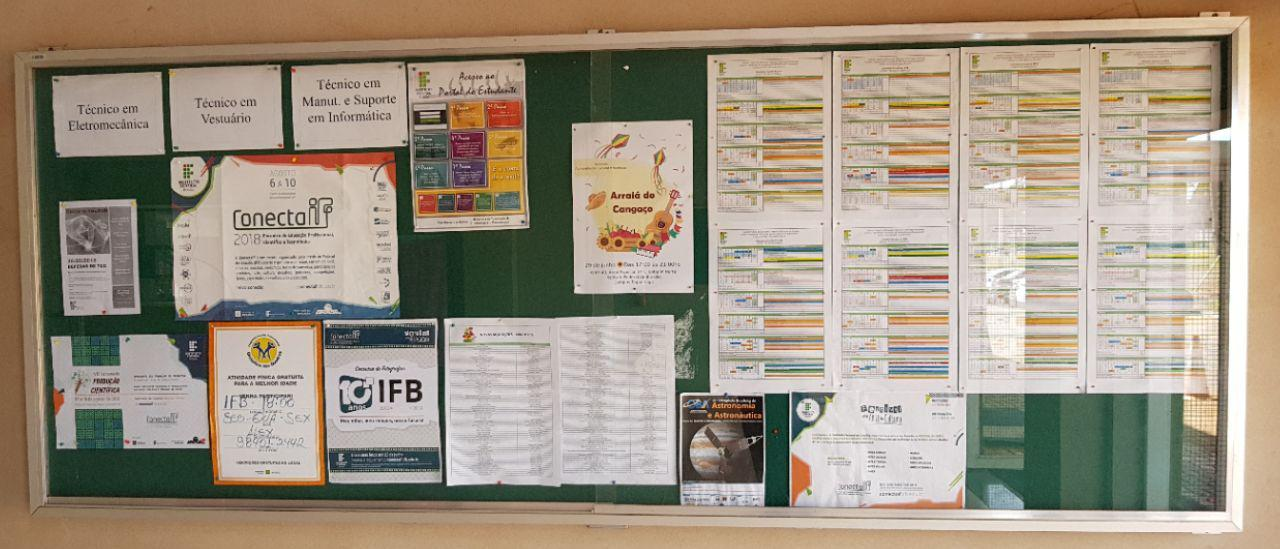
\includegraphics[height=3cm]{figuras/paineis.png}
    \label{fig3b}
  }
  \caption{Meios de divulgação fisicamente}
\label{fig1}
\end{figure}
\end{frame}

\begin{frame}{Quais são os problemas?}
\begin{itemize}
   \item Falta de integração entre os veículos de comunicação;
   \vspace{10px}
   \item Falta de interatividade com as notícias;
   \vspace{10px}
   \item Má disseminação da notícia;
   \vspace{10px}
   \item Difícil acesso;
\end{itemize}	 
\end{frame}

\subsection{Proposta}
\begin{frame}{Propostas}
	\begin{itemize}
		\item Usar o SIDv2 como base para implementação da versão 3;
		\vspace{10px}
		\item Dinamizar a criação e edição das publicações;
		\vspace{10px}
		\item Unir os conceitos de marketing digital e sinalização digital, para melhoria na exposição e interação com a notícia;
		\vspace{10px}
		\item Integrar os atuais sistemas de divulgação;
		\vspace{10px}
		\item Aplicativo mobile que apresente as publicações e oferece forma de interação entre professores e alunos com a simulação de algumas funcionalidades de um Sistema de Gestão Acadêmia.
	\end{itemize}
\end{frame}

\subsection{Objetivos}
\begin{frame}{Objetivos}
	\begin{itemize}
   		\item Levantamento de requisitos de sistemas que usam sinalização e marketing digital;
   		\vspace{10px}
   		\item Estudo da documentação da Graph API;
   		\vspace{10px}
   		\item Definição e implementação do SIDv3 e do aplicativo mobile;
   		\vspace{10px}
   		\item Criação da documentação do software;
   		\vspace{10px}
   		\item Aplicativo mobile com consumo de uma API fictícia para posterior integração;
	\end{itemize}
\end{frame}

\begin{frame}{Objetivos específicos}
	\begin{itemize}
   		\item Estudo de Frameworks mobile e PHP;
   		\vspace{10px}
   		\item Implementação de uma API REST;
   		\vspace{10px}
   		\item Sugestão de propostas de implantações;
	\end{itemize}
\end{frame}

\subsection{Metodologia}
\begin{frame}{Metodologia}
	\begin{itemize}
   		\item Realizar uma revisão da bibliografia;
   		\vspace{10px}
   		\item Avaliar os pontos negativos das ferramentas testadas, baseando-se nas necessidades do Campus;
   		\vspace{10px}
   		\item Estudar a documentação da Graph API e suas ferramentas;
   		\vspace{10px}
   		\item Estudo dos Frameworks mobile e PHP;
   		\vspace{10px}
   		\item Realizar as modificações que forem necessárias e não implementadas na segunda versão do SID.
   		\vspace{10px}
   		\item Seguir os conceitos de desenvolvimento ágil, com metodologia SCRUM, Realizando sprints semanais para apresentação das melhorias;
	\end{itemize}
\end{frame}

\section{Trabalhos Relacionados} 
\begin{frame}{Trabalhos relacionados}
	\begin{figure}[h]
    	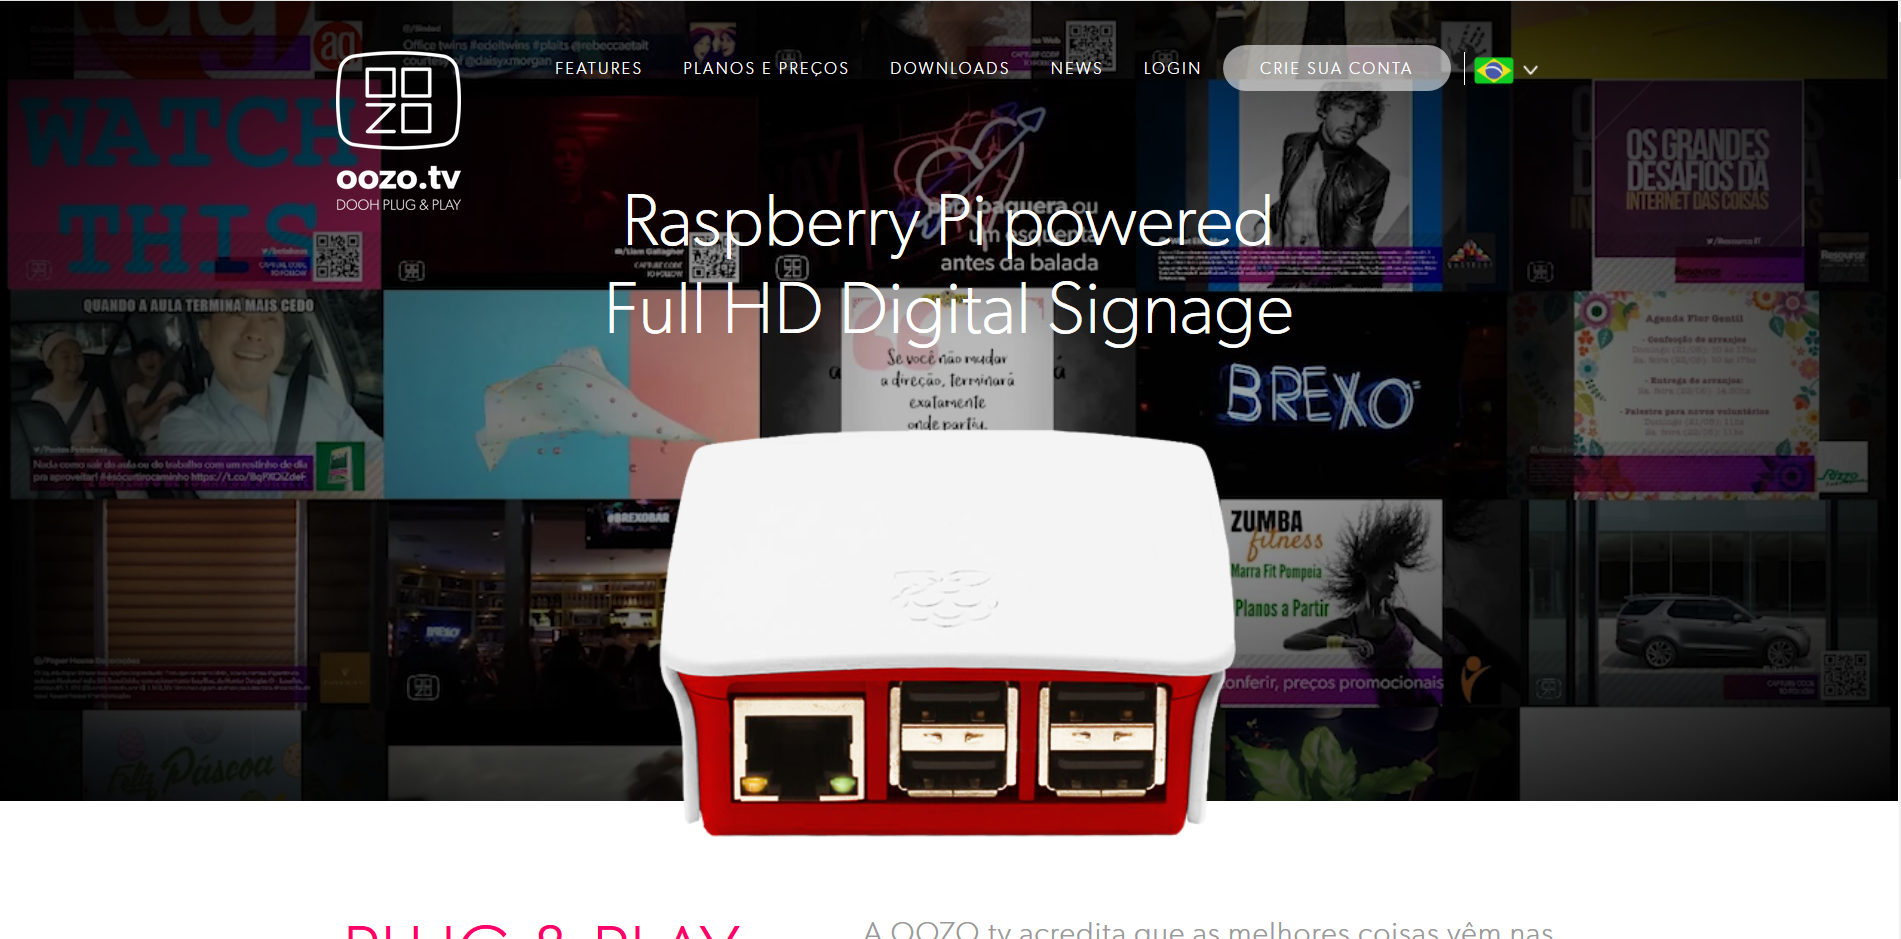
\includegraphics[height=4cm]{figuras/oozo.png}
    	\caption{Oozo}
	\end{figure}
	\begin{center}
	Além da versão gratuita possuir limitações de não possuir filtro e não publicar vídeos, ele não exibe comentários, não possui aplicativo mobile e não publica diretamente no Facebook.
	\end{center}
\end{frame}

\begin{frame}{Trabalhos relacionados}
	\begin{figure}[h]
    	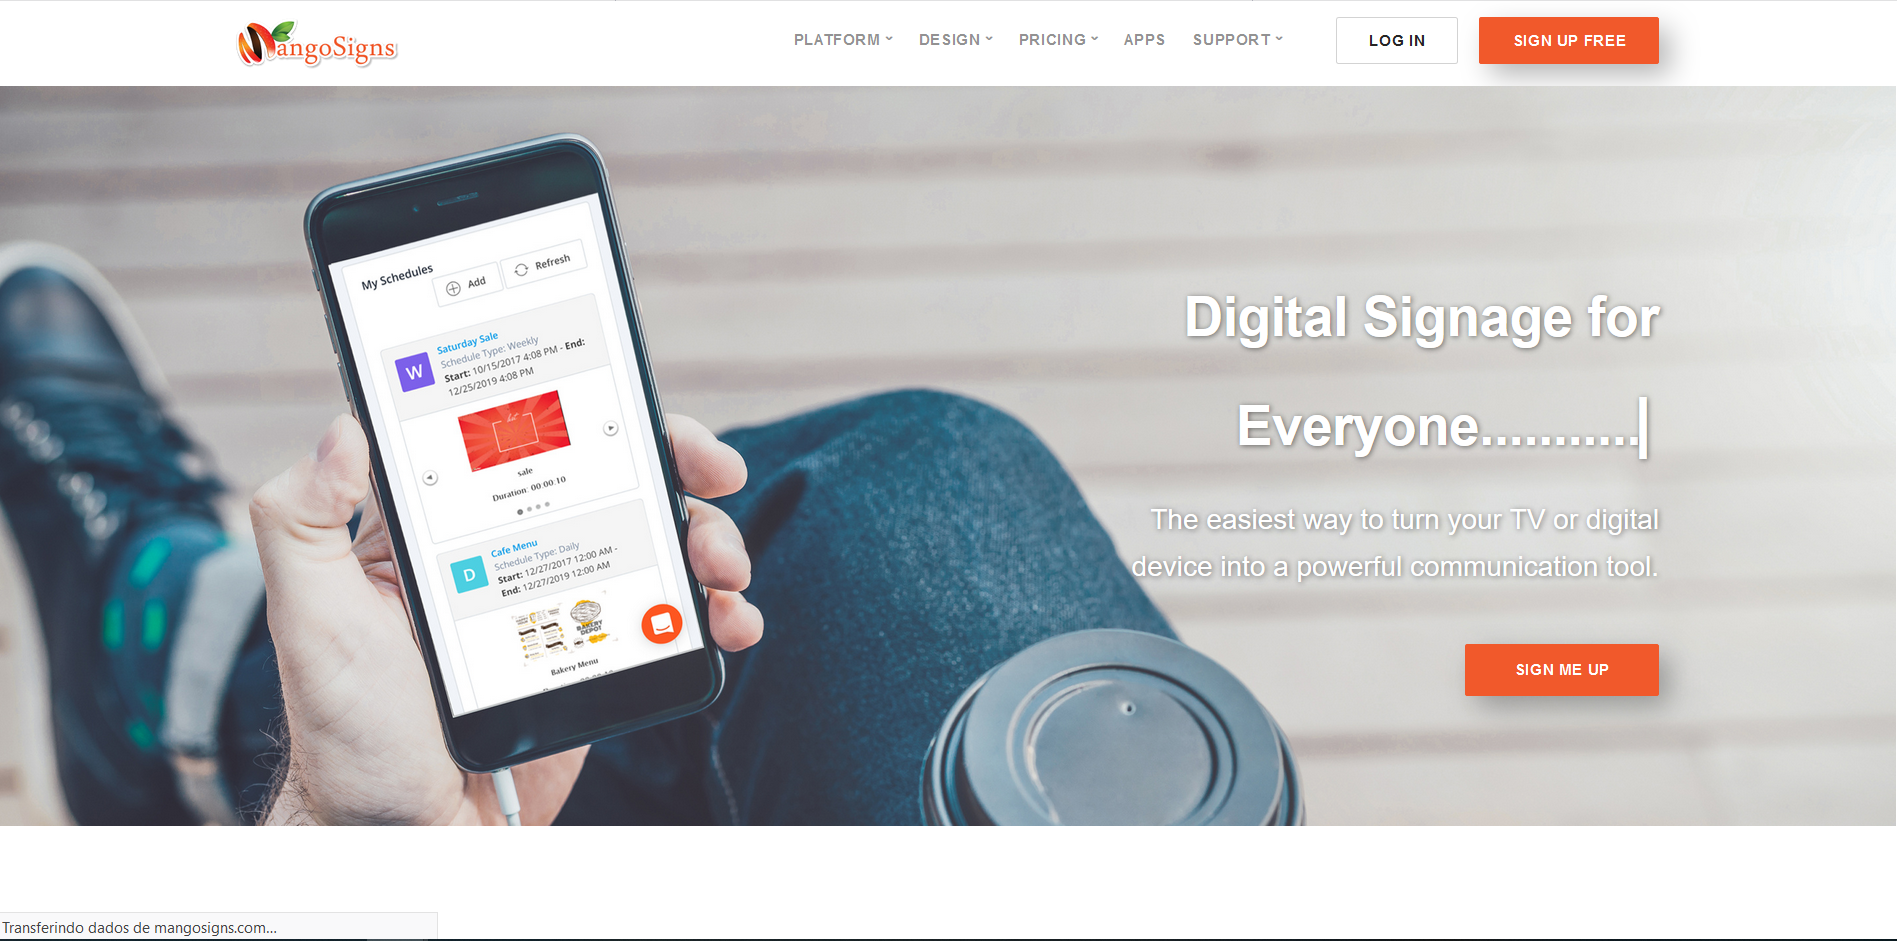
\includegraphics[height=4cm]{figuras/mango.png}
    	\caption{Mango Signs}
	\end{figure}
	\begin{center}
	Além da versão gratuita não possuir integração com o Facebook, ele não oferece leitura por QR Code e limita a 3 imagens.
	\end{center}
\end{frame}

\begin{frame}{Trabalhos relacionados}
	\begin{figure}[h]
    	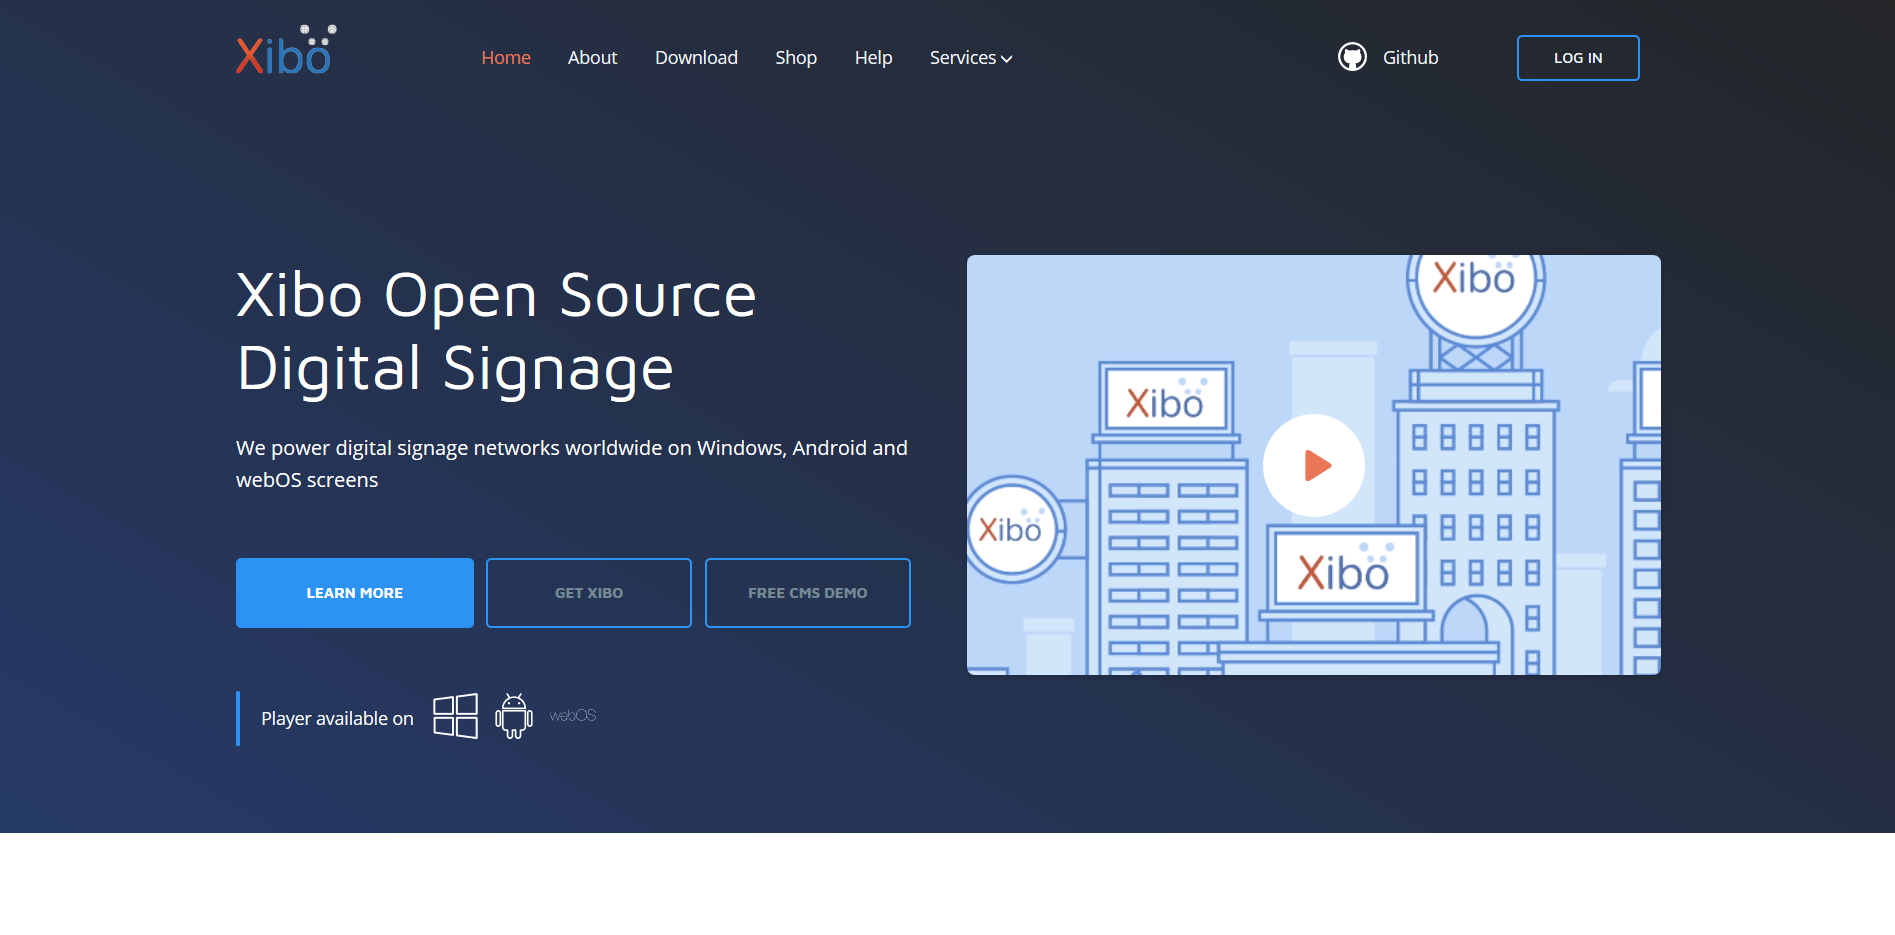
\includegraphics[height=4cm]{figuras/xibo.png}
    	\caption{Xibo}
	\end{figure}
	\begin{center}
	Não oferece integração com nenhuma rede social, além de complicada criação de nova publicação.
	\end{center}
\end{frame}

\begin{frame}{Trabalhos relacionados}
	\begin{figure}[h]
    	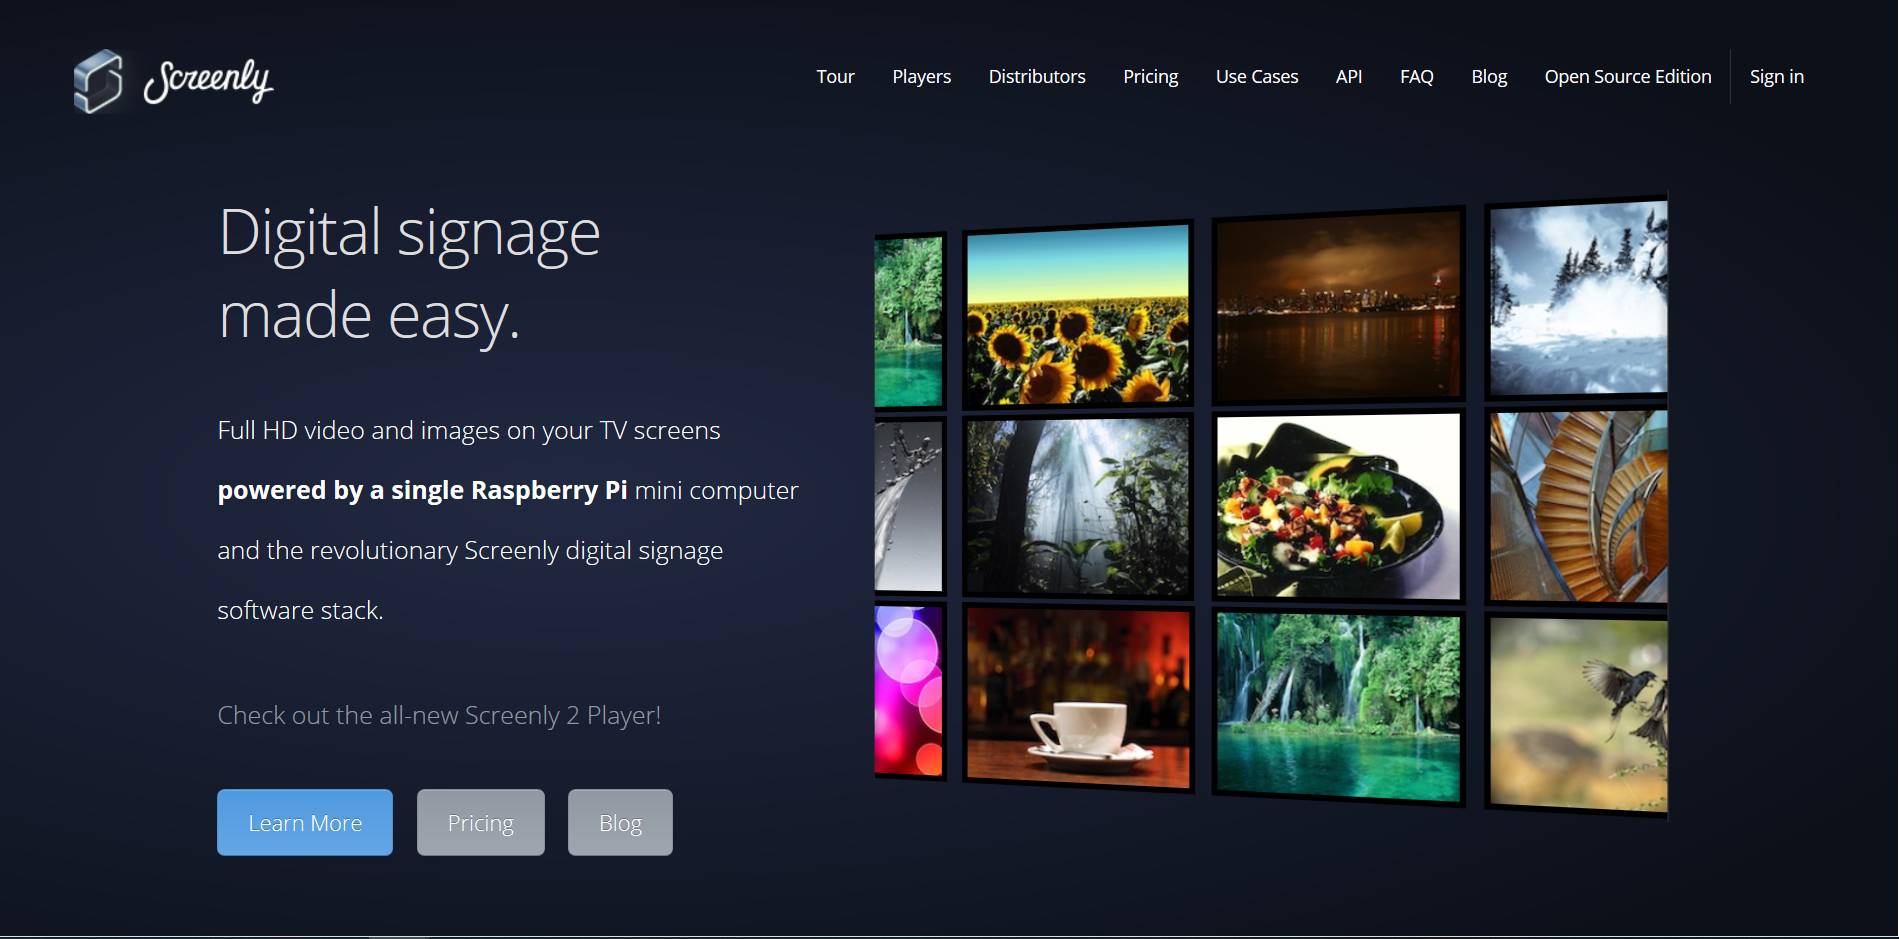
\includegraphics[height=4cm]{figuras/screenly.png}
    	\caption{Screenly}
	\end{figure}
	\begin{center}
	Limitações de exibição na versão gratuita e sem nenhuma integração.
	\end{center}
\end{frame}

\begin{frame}{Trabalhos relacionados}
\begin{figure}[h]
    	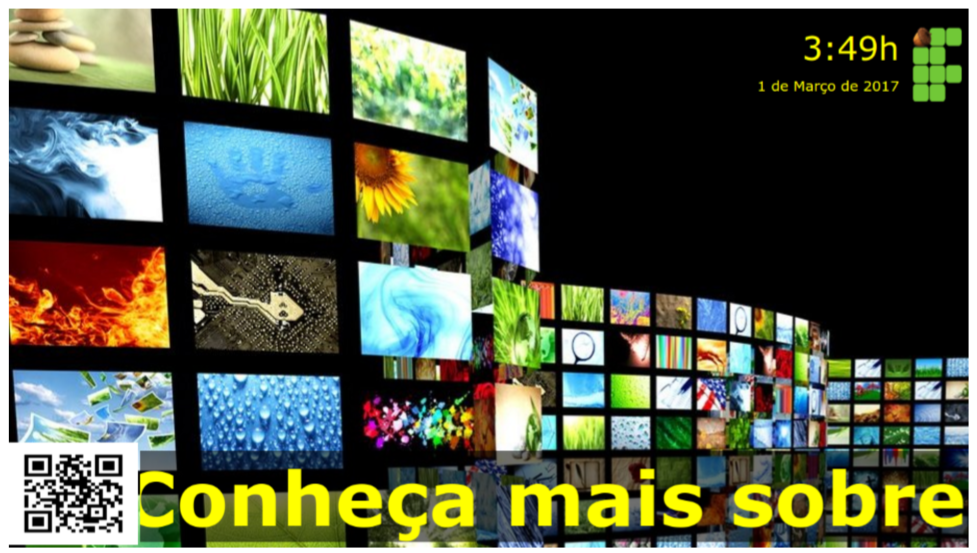
\includegraphics[height=3cm]{figuras/SID.png}
    	\caption{Screenly}
	\end{figure}
	
	\begin{center}
O SIDv2 (SID FORMOSA), trabalho utilizado como base para melhorias no sistema. Além de possuir não possuir uma integração completa com o Facebook, o link para o QRCode deve ser colocado manualmente, não oferece possibilidade de colocar data de início e não possuir aplicação mobile.
\end{center}
\end{frame}

\section{Graph API}
\begin{frame}{Graph API}
	\begin{center}
	Integrar o Facebook a outros aplicativos externos. Com o uso dela é possível realizar as requisições de dados para a rede social.\\
	\vspace{20px}
	Utiliza-se dos conceitos de grafos, onde possui vértice, aresta e campo. Um Grafo é um conjunto finito de vértices e cada par de vértices relacionado é chamado de aresta. \\
	\vspace{20px}
	Segue a estrutura REST, possibilitando requisições HTTP do tipo GET, POST e DELETE. 
	\end{center}
\end{frame}

\begin{frame}{Estrutura}
	\begin{figure}[h]
		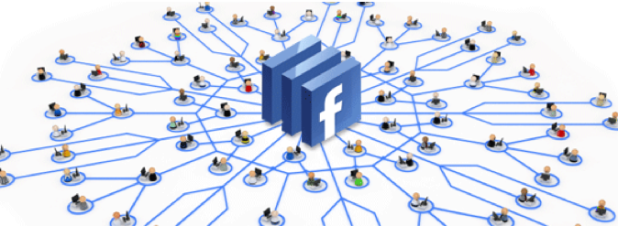
\includegraphics[width=8cm]{figuras/facebookgraph.png}
		\caption{Graph Api \cite{figura3}}
		\label{fig:facebookgraph}
	\end{figure}
\end{frame}

\begin{frame}{Requisição de dados}
\begin{figure}[h]
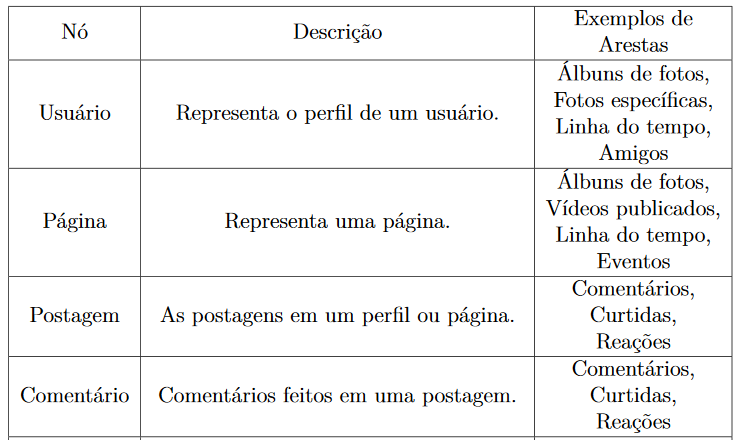
\includegraphics[width=10cm]{figuras/nosarestas.png}
\label{fig:facebookgraph}
\end{figure}
\end{frame}

\begin{frame}{Requisição de dados}
\begin{figure}[h]
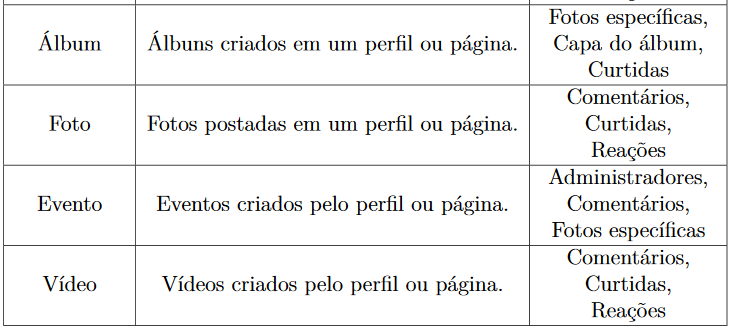
\includegraphics[width=10cm]{figuras/nosarestas2.png}
\label{fig:facebookgraph}
\end{figure}
\end{frame}

\begin{frame}{Detalhes}
\begin{itemize}
   \item Necessário um Token;
   \item Autenticação em conformidade com protocolo OAuth 2.0;
   \item Acesso de acordo com as permissões concedidas;
\end{itemize}
\end{frame}

\begin{frame}{Tipos de requisição}
\begin{figure}[h]
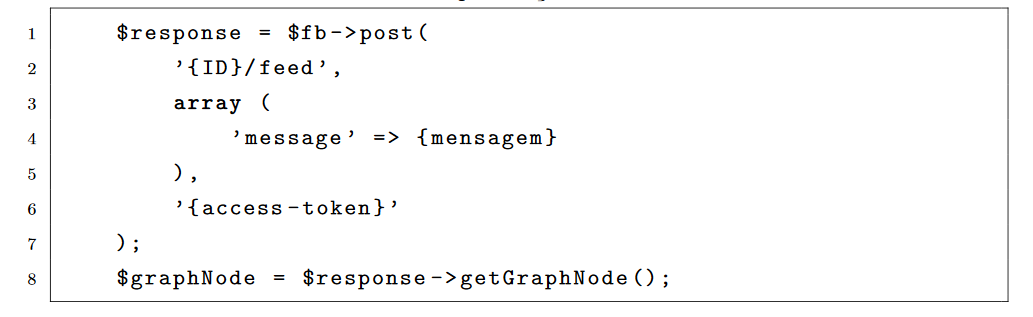
\includegraphics[width=10cm]{figuras/requisicaopost.png}
\label{fig:facebookgraph}
\end{figure}
\begin{figure}[h]
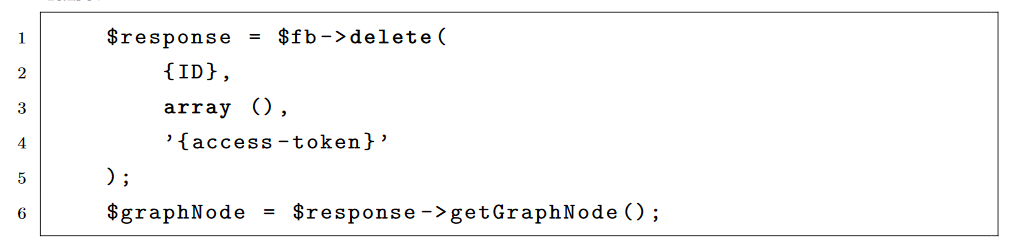
\includegraphics[width=10cm]{figuras/requisicaodelete.png}
\label{fig:facebookgraph}
\end{figure}
\end{frame}

\begin{frame}{Formas de Requisições}
\begin{figure}[h]
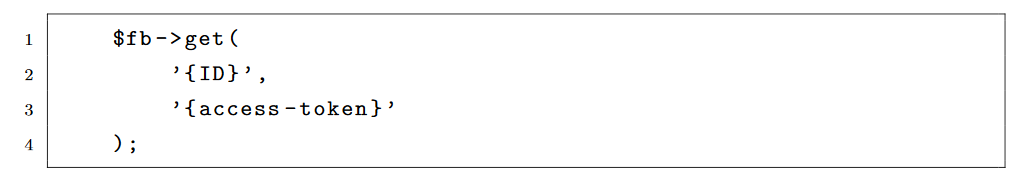
\includegraphics[width=10cm]{figuras/requisicaovertice.png}
\label{fig:facebookgraph}
\end{figure}

\begin{figure}[h]
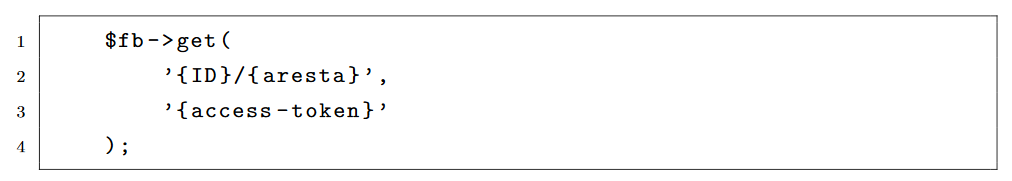
\includegraphics[width=10cm]{figuras/requisicaoaresta.png}
\label{fig:facebookgraph}
\end{figure}

\begin{figure}[h]
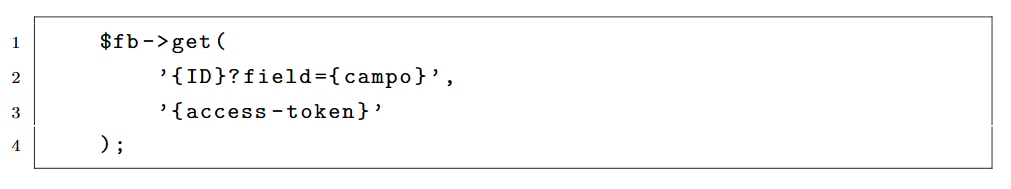
\includegraphics[width=10cm]{figuras/requisicaocampo.png}
\label{fig:facebookgraph}
\end{figure}
\end{frame}

\begin{frame}{Requisição na pratica}
	\begin{figure}[h]
		
\includegraphics[width=10cm]{figuras/requisicao3.png}
		\label{fig:facebookgraph}
	\end{figure}

	\begin{figure}[h]
		
\includegraphics[width=10cm]{figuras/requisicao1.png}
		\label{fig:facebookgraph}
	\end{figure}
	
	\begin{figure}[h]
		
\includegraphics[width=10cm]{figuras/requisicao4.png}
		\label{fig:facebookgraph}
	\end{figure}
	
	\begin{figure}[h]
		
\includegraphics[width=10cm]{figuras/requisicao5.png}
		\label{fig:facebookgraph}
	\end{figure}
\end{frame}

\begin{frame}{Retorno das requisição}
\begin{figure}[h]
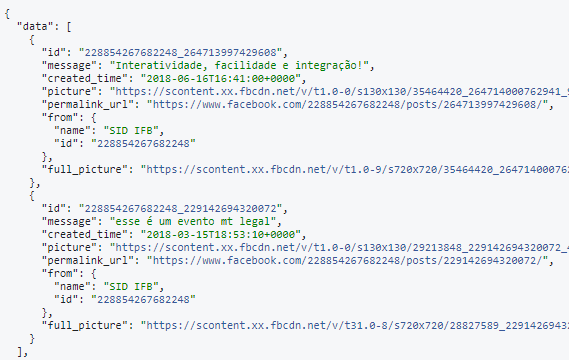
\includegraphics[width=10cm]{figuras/requisicao2.png}
\label{fig:facebookgraph}
\end{figure}
\end{frame}

\section{SID}
\begin{frame}
\begin{center}
Sistema Integrado de Divulgação (Versão 3)
\end{center}
\end{frame}
\subsection{Modulos}
\subsubsection{Administrador}
\begin{frame}{Administrador}
Situado no servidor e com acesso restrito, é responsável por conceder ao usuário administrador as funcionalidades de gerenciamento do sistema, tais como:
\begin{itemize}
   \item Inserção;
   \item Listagem;
   \item Detalhamento;
   \item Exclusão;
   \item Edição;
\end{itemize}
\end{frame}

\begin{frame}{Submódulo API}
Situado no servidor, é responsável por:
	\begin{itemize}
		\item Fornecer uma estrutura REST para possíveis requisições HTTP do tipo GET, POST, UPDATE e DELETE.
		\vspace{10px}
   		\item Recuperação dos dados armazenados no banco e no Facebook;
   		\vspace{10px}
   		\item Tratamento e formatação dos dados recuperados, para envio ao cliente quando requisitado;
   		\vspace{10px}
   		\item Simular parte das funcionalidades de um Sistema de Gestão Acadêmcica, para que seja possível o consumo dos dados por um aplicativo externo, via API.
	\end{itemize}
\end{frame}

\subsubsection{Cliente}
\begin{frame}{Módulo Cliente}
Podendo ser situado no servidor ou em um dispositivo externo, como um Raspeberry, para exibição em monitores e televisões, ele é responsável por:
\begin{itemize}
   \item Realizar requisições ao submódulo API para obter os dados;
   \vspace{10px}
   \item Exibir de forma simples e dinâmica os dados recebidos;
   \vspace{10px}
   \item Realizar a troca do conteúdo que está sendo exibido de acordo com o tempo definido;
   \vspace{10px}
   \item Oferecer acesso a publicação completa via QRCode;
\end{itemize}
\end{frame}

\subsubsection{Mobile}
\begin{frame}{Mobile}
Proposta de aplicativo mobile que é responsável por:
\begin{itemize}
   \item Realizar requisições ao submódulo API para obter os dados;
   \vspace{10px}
   \item Exibir de forma simples e dinâmica os dados recebidos;
   \vspace{10px}
   \item Realizar a troca do conteúdo que está sendo exibido de acordo com o tempo definido;
   \vspace{10px}
   \item Simular o consumo de uma API para trocar de mensagem entre a comunidade acadêmica;
\end{itemize}
\end{frame}

\subsection{Apresentação}
\begin{frame}{Apresentação Facebook}
\begin{figure}[h]
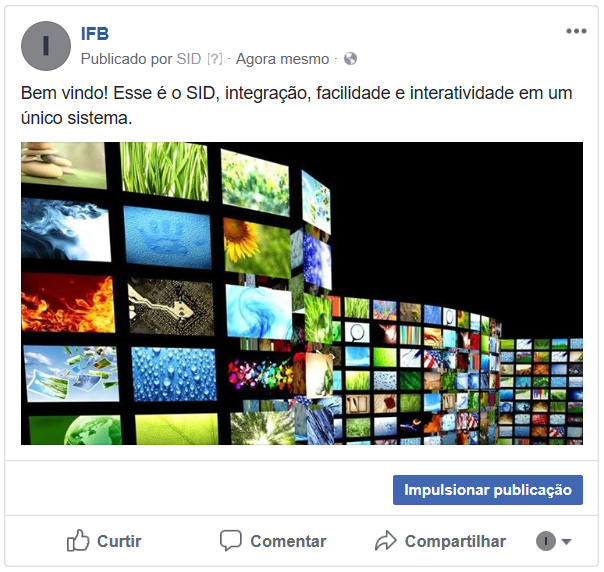
\includegraphics[width=7cm]{figuras/imgfacebook1.png}
\label{fig:facebookgraph}
\end{figure}
\end{frame}

\begin{frame}{Apresentação Modulo Cliente}
\begin{figure}[h]
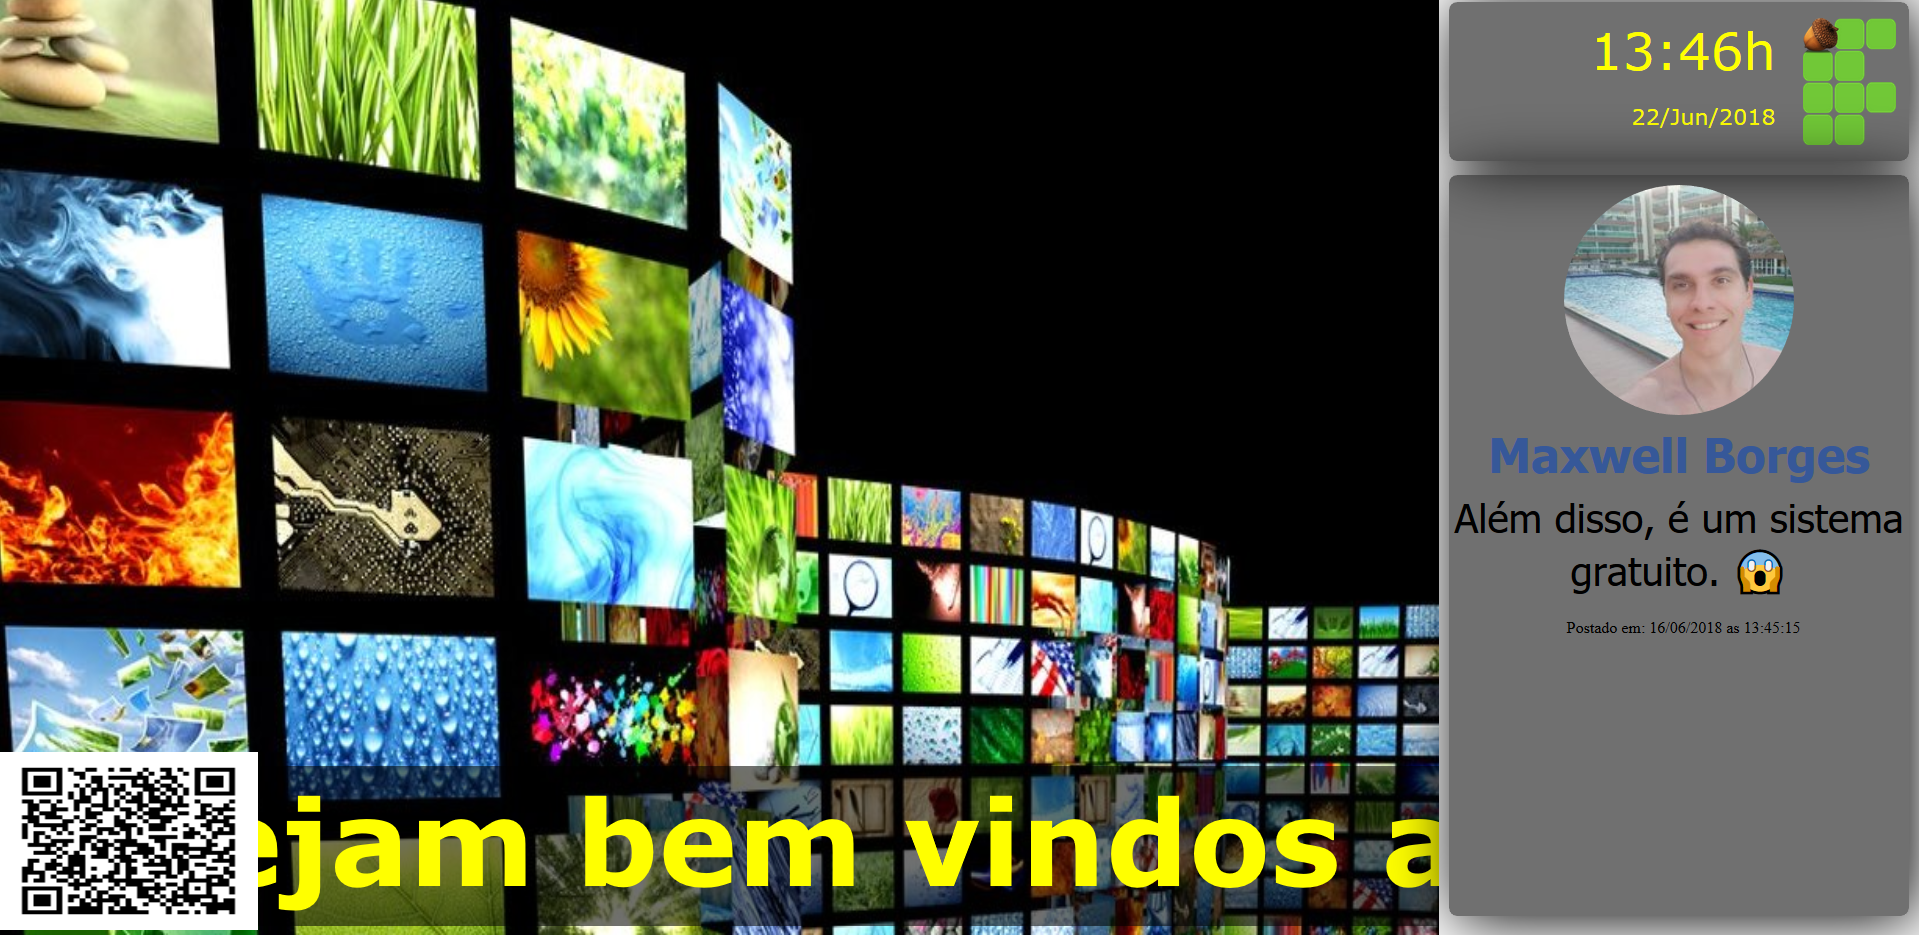
\includegraphics[width=11cm]{figuras/funcionalidadeexibir.png}
\label{fig:facebookgraph}
\end{figure}
\end{frame}

\begin{frame}{Apresentação Aplicativo}
	\begin{figure}[h]
    	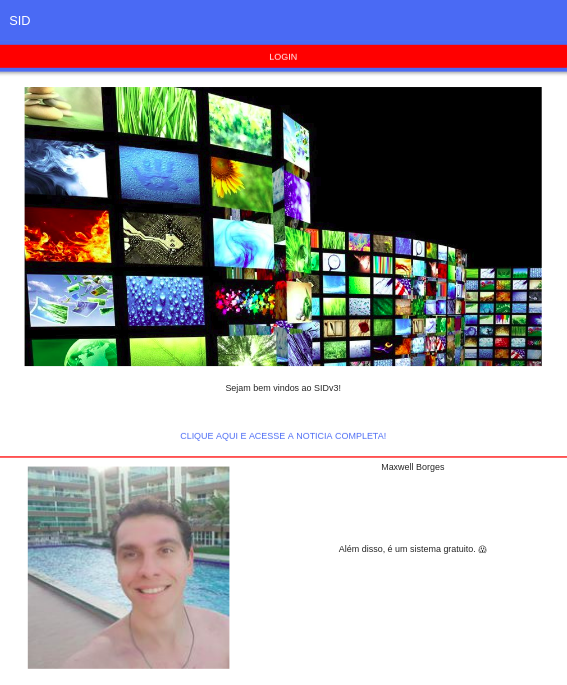
\includegraphics[height=6cm]{figuras/mobile1.png}
	\end{figure}
\end{frame}



\section{Resultados}
\begin{frame}{Características comparadas}
	\begin{enumerate}
		\item Comprometimento com o propósito;
		\item Criação simples de divulgações;
		\item Portabilidade mobile;
		\item Integração com redes sociais; (Comentários e likes)
		\item Sem limitações na versão gratuita;
		\item Criação e envio para as redes sociais;
	\end{enumerate}
	\begin{figure}[h]
		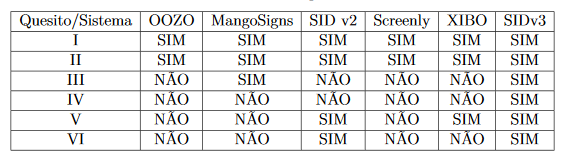
\includegraphics[width=10cm]{figuras/tabela.png}
		\label{fig:figuramobile3}
	\end{figure}
\end{frame}

\section{Conclusão e trabalhos futuros}
\begin{frame}{Conclusão}
\begin{center}
O SID apresenta benefícios consideravelmente melhores em relação às outras soluções que são utilizadas atualmente, além da divisão entre módulos possibilitar a exibição das divulgações em diversos dispositivos distintos, incluindo o aplicativo mobile que foi desenvolvido.
\end{center}
\end{frame}

\begin{frame}{Conclusão}
\begin{itemize}
\item Integração completa;
\item Divulgação intuitiva;
\item unificação de dois meios de comunicação distinto;
\item Consumo de uma API Fictícia para posterior integração com SGA;
\end{itemize}
\end{frame}


\begin{frame}{Trabalhos Futuros}
\begin{itemize}
\item Finalização do aplicativo mobile;
\item Melhoria na moderação de comentários;
\item Atraso na recuperação de dados;
\end{itemize}
\end{frame}

\section{bibliografia}
\begin{frame}[allowframebreaks]
\bibliographystyle{apalike}
\bibliography{bibliografia}
\end{frame}
\end{document}